\appendix
\section{Mixed-Integer Linear Programming Model}




\section{Novel Metrics}



\begin{figure*}[h]
     \centering
          \begin{subfigure}[b]{0.32\linewidth}
         \centering
         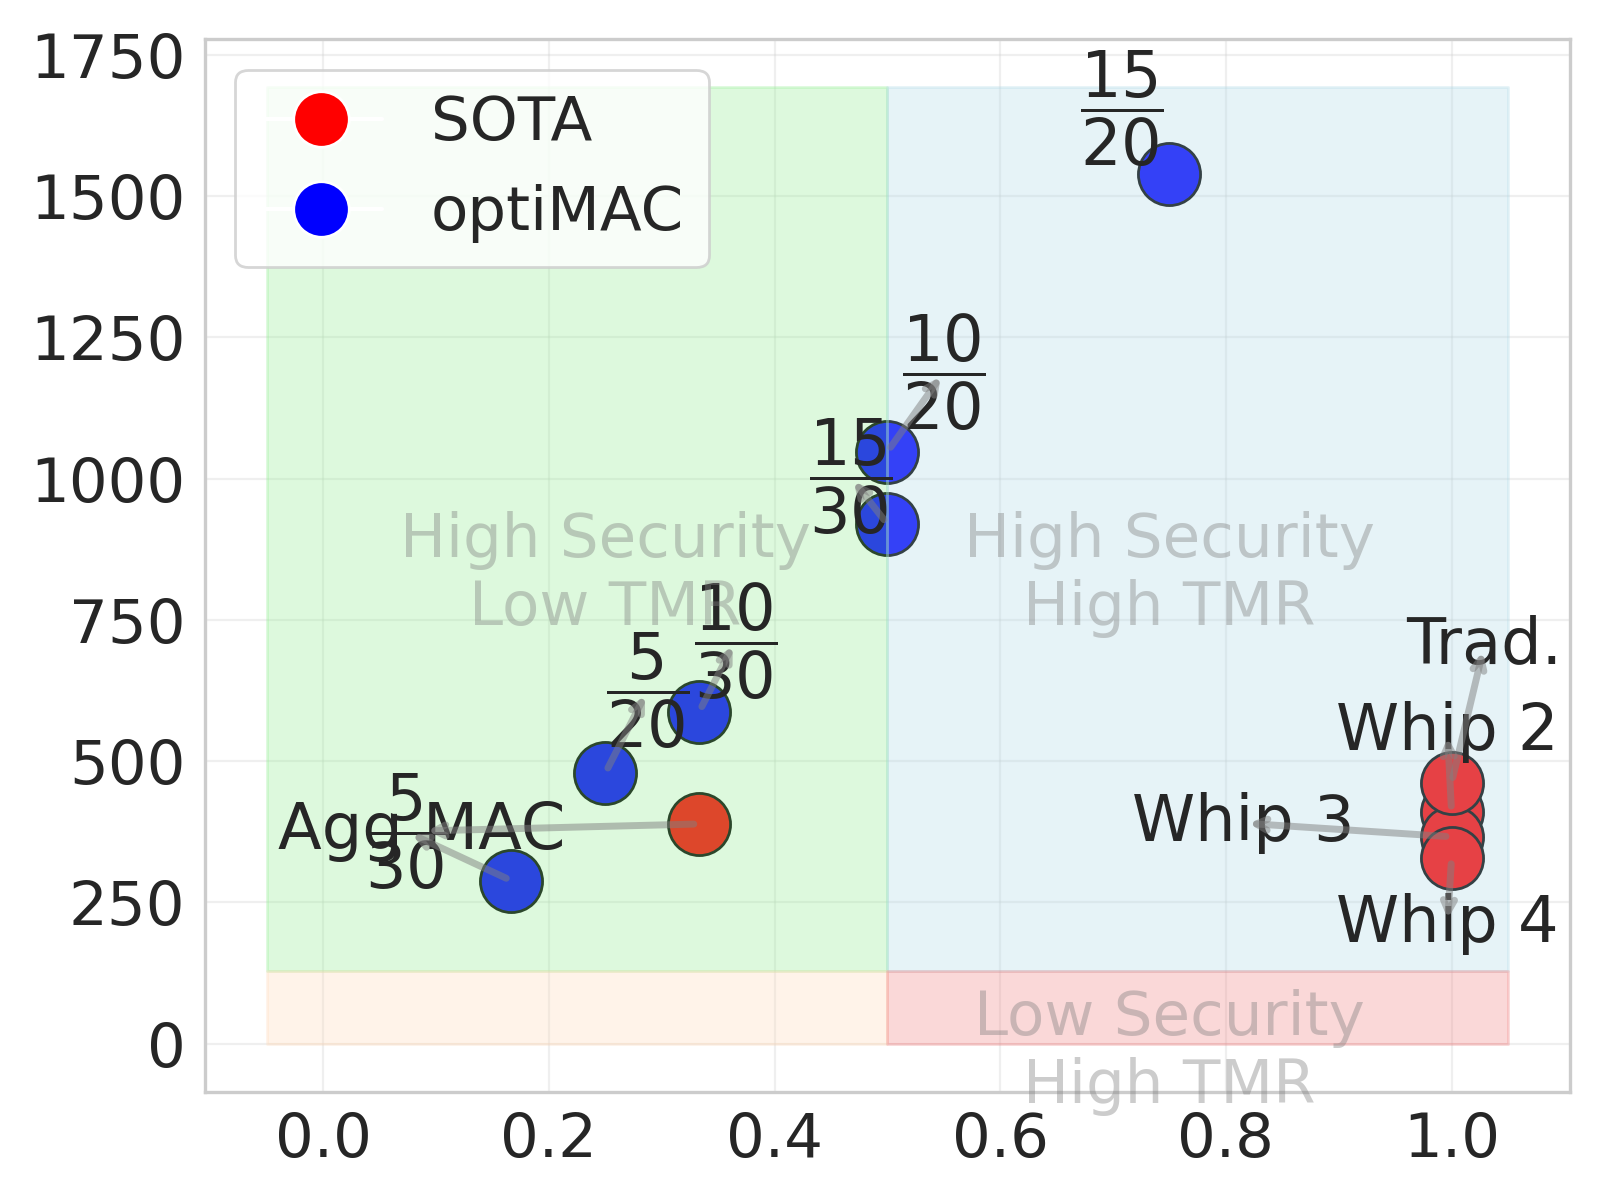
\includegraphics[width=\linewidth]{img/results/5G/0.1S'.png}
         \caption{Attack rate 0.1}
         \label{fig:0.1S 5G}
     \end{subfigure} \hfill
     \begin{subfigure}[b]{0.32\linewidth}
         \centering
         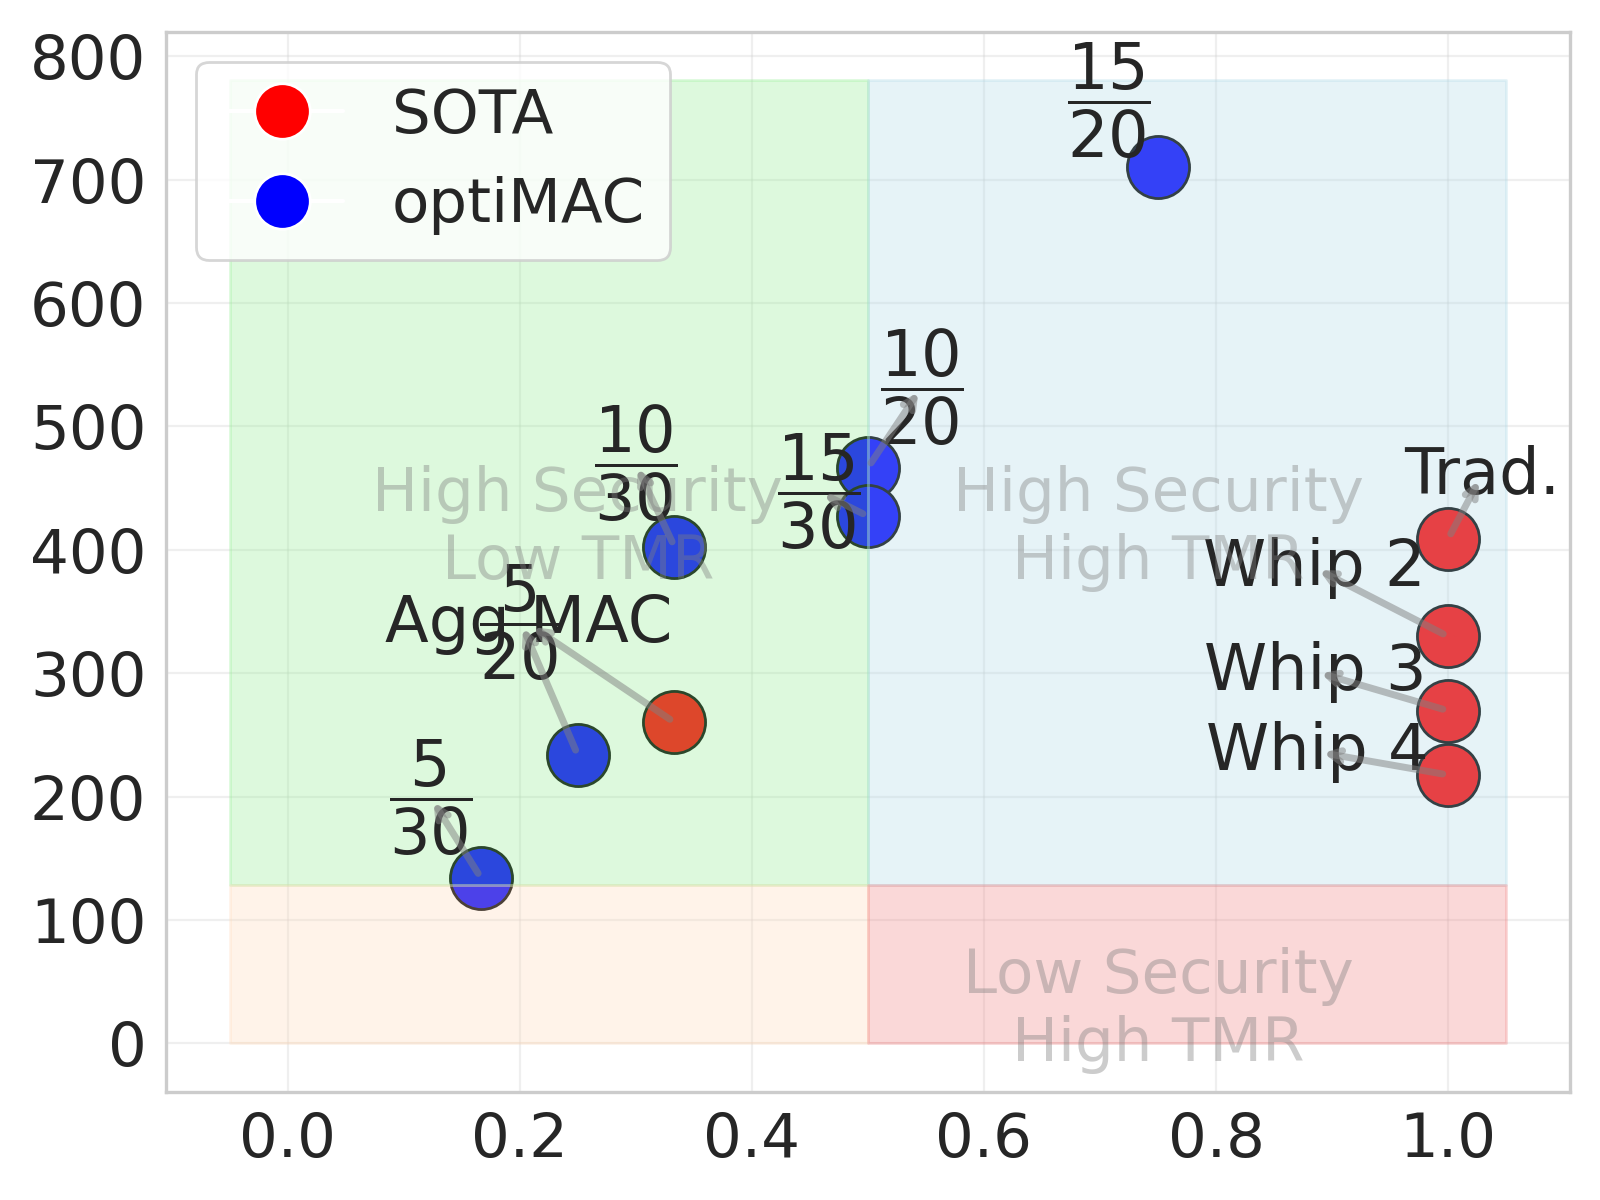
\includegraphics[width=\linewidth]{img/results/5G/0.2S'.png}
         \caption{Attack rate 0.2}
         \label{fig:0.2S 5G}
     \end{subfigure}
     \hfill
      \begin{subfigure}[b]{0.32\linewidth}
         \centering
         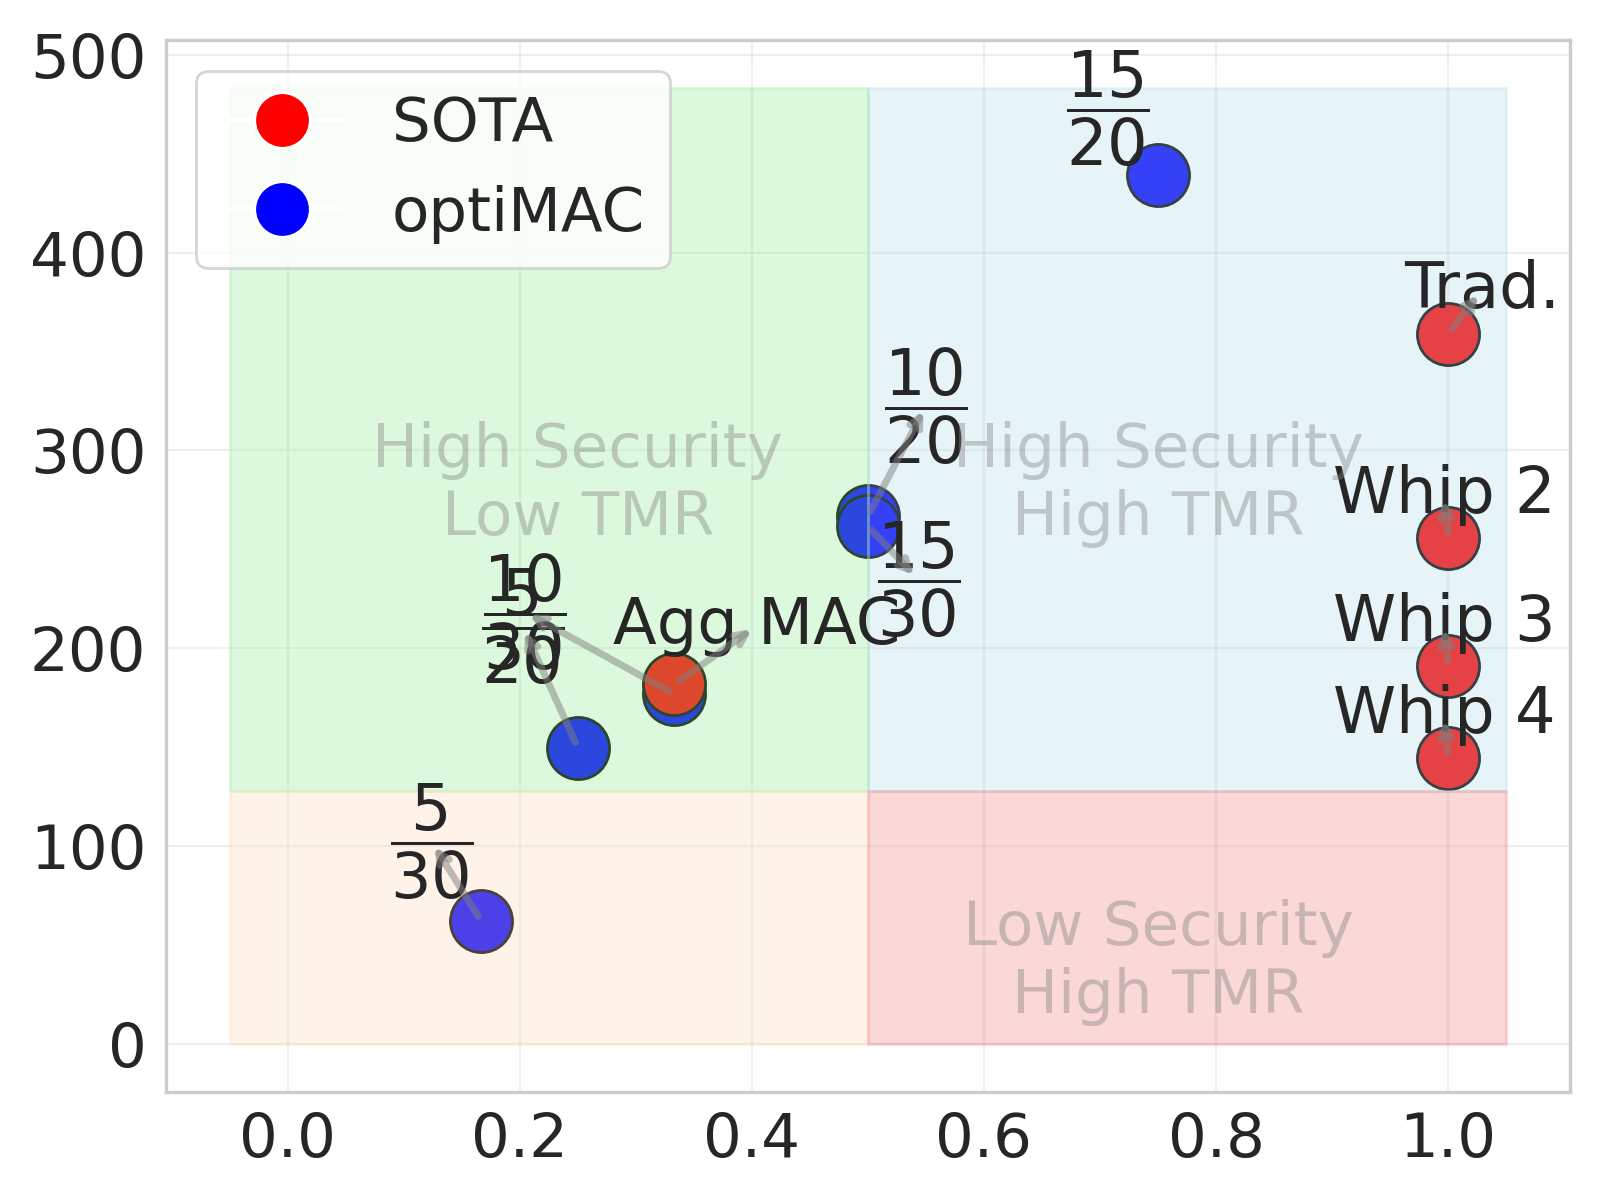
\includegraphics[width=\linewidth]{img/results/5G/0.3S'.png}
         \caption{Attack rate 0.3}
         \label{fig:0.3S 5G}
     \end{subfigure}

     \caption{TbpM (y-axis) vs. TMR (x-axis) of 5G experiments with 512-bit tags (256 or higher TbpM is high security). State-of-the-art (SOTA) includes traditional, progressive, and aggregate MAC vs. the optiMAC.}
     \label{fig:Security5G}
\end{figure*}

\begin{figure*}[h]
     \centering
          \begin{subfigure}[b]{0.32\linewidth}
         \centering
         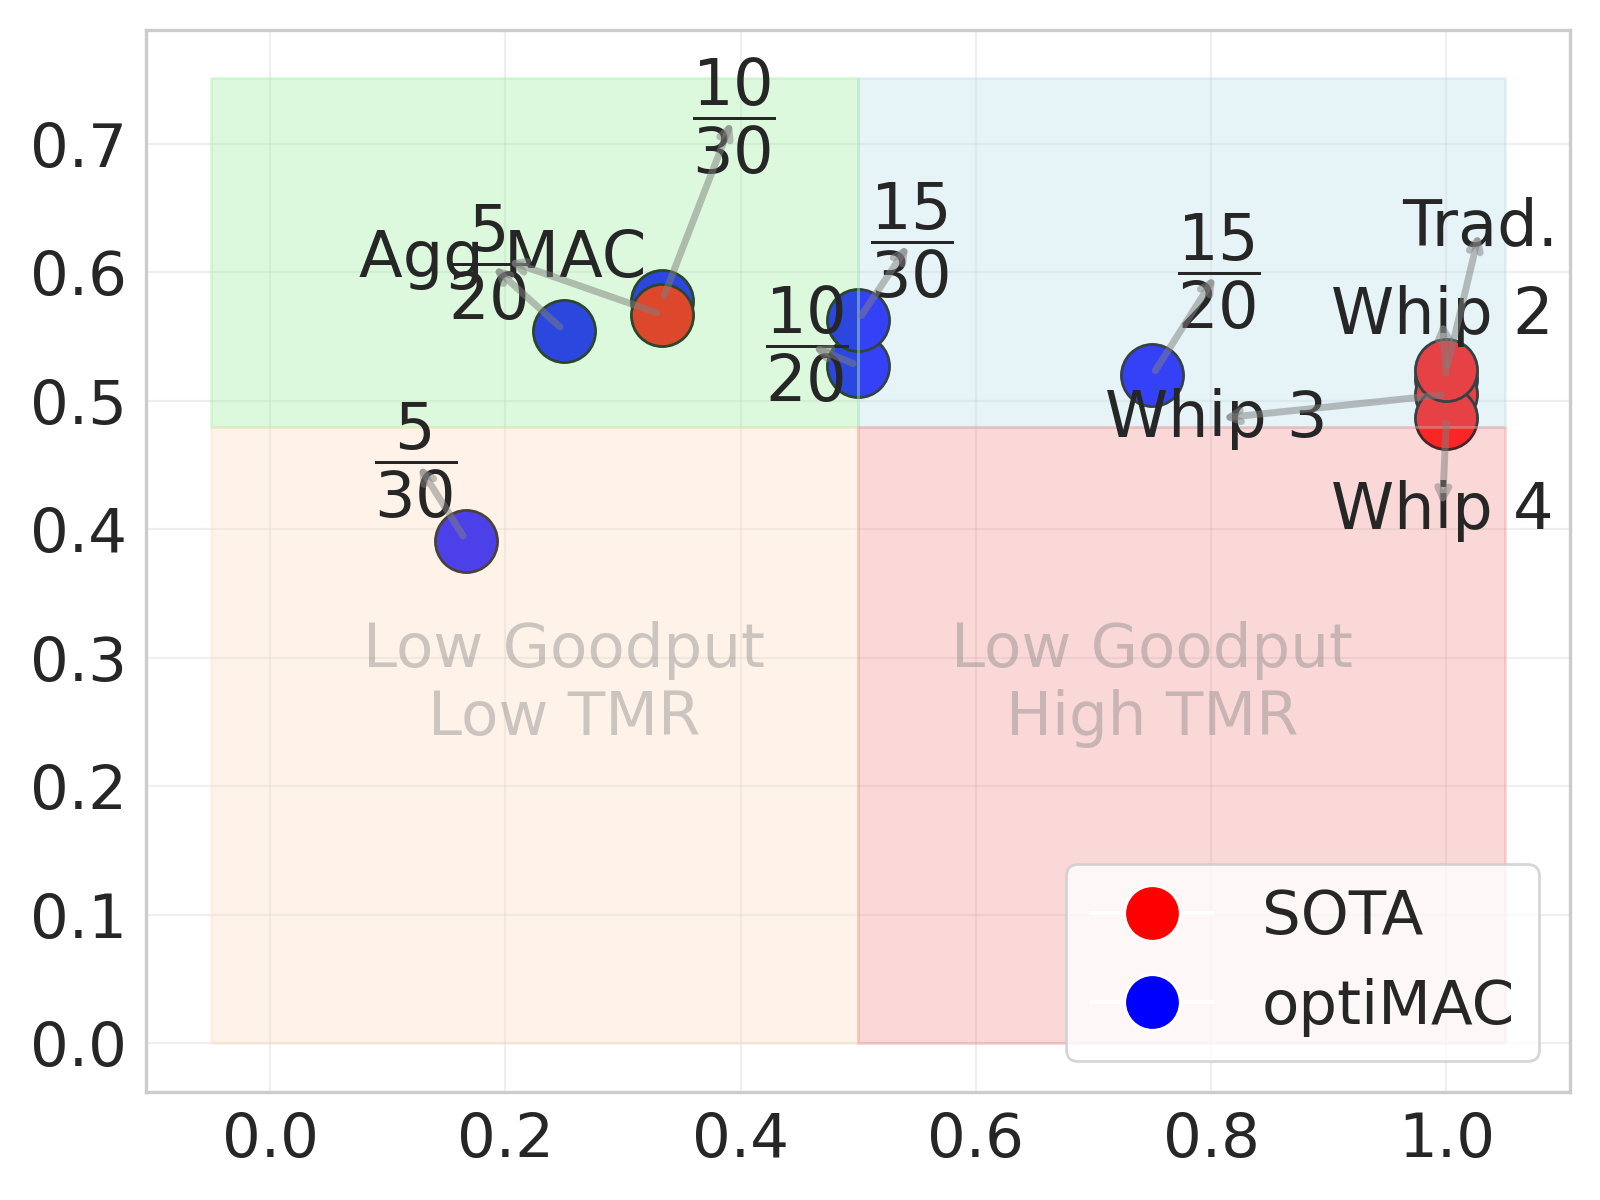
\includegraphics[width=\linewidth]{img/results/5G/0.1G'.png}
         \caption{Attack rate 0.1}
         \label{fig:0.1G 5G}
     \end{subfigure} \hfill
     \begin{subfigure}[b]{0.32\linewidth}
         \centering
         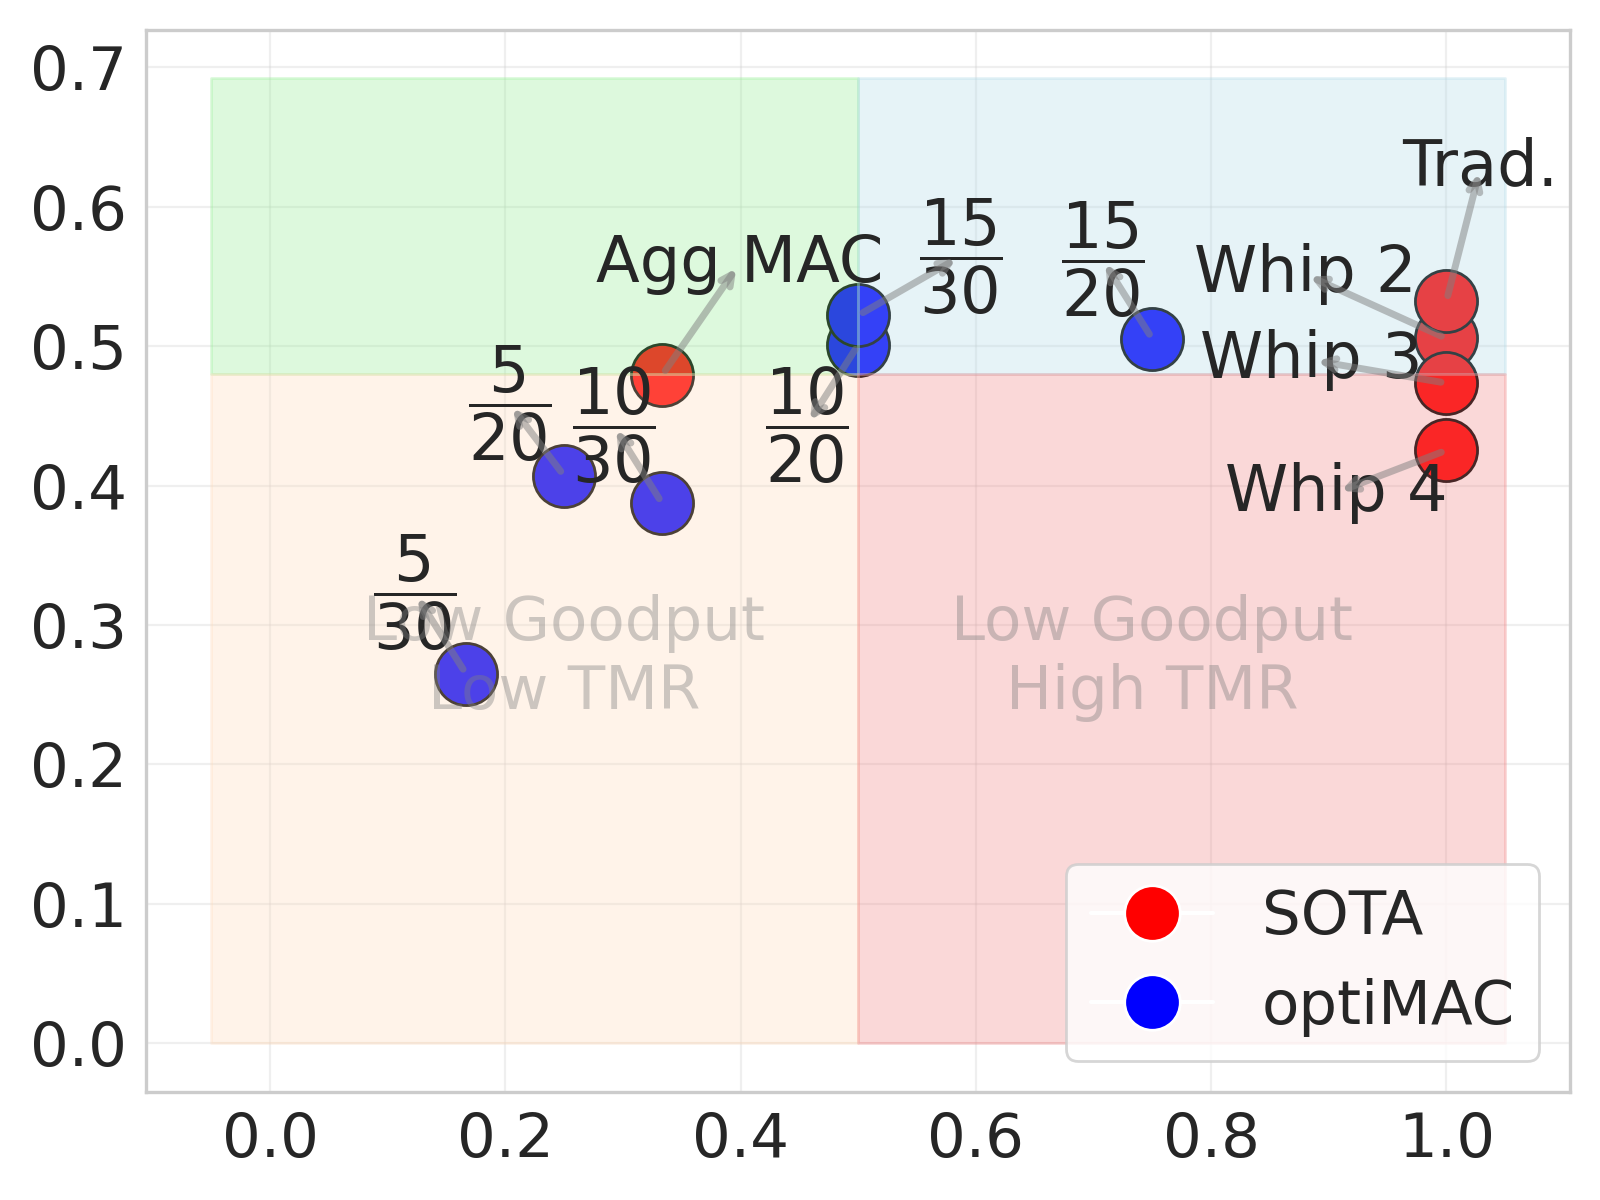
\includegraphics[width=\linewidth]{img/results/5G/0.2G'.png}
         \caption{Attack rate 0.2}
         \label{fig:0.2G 5G}
     \end{subfigure}
     \hfill
      \begin{subfigure}[b]{0.32\linewidth}
         \centering
         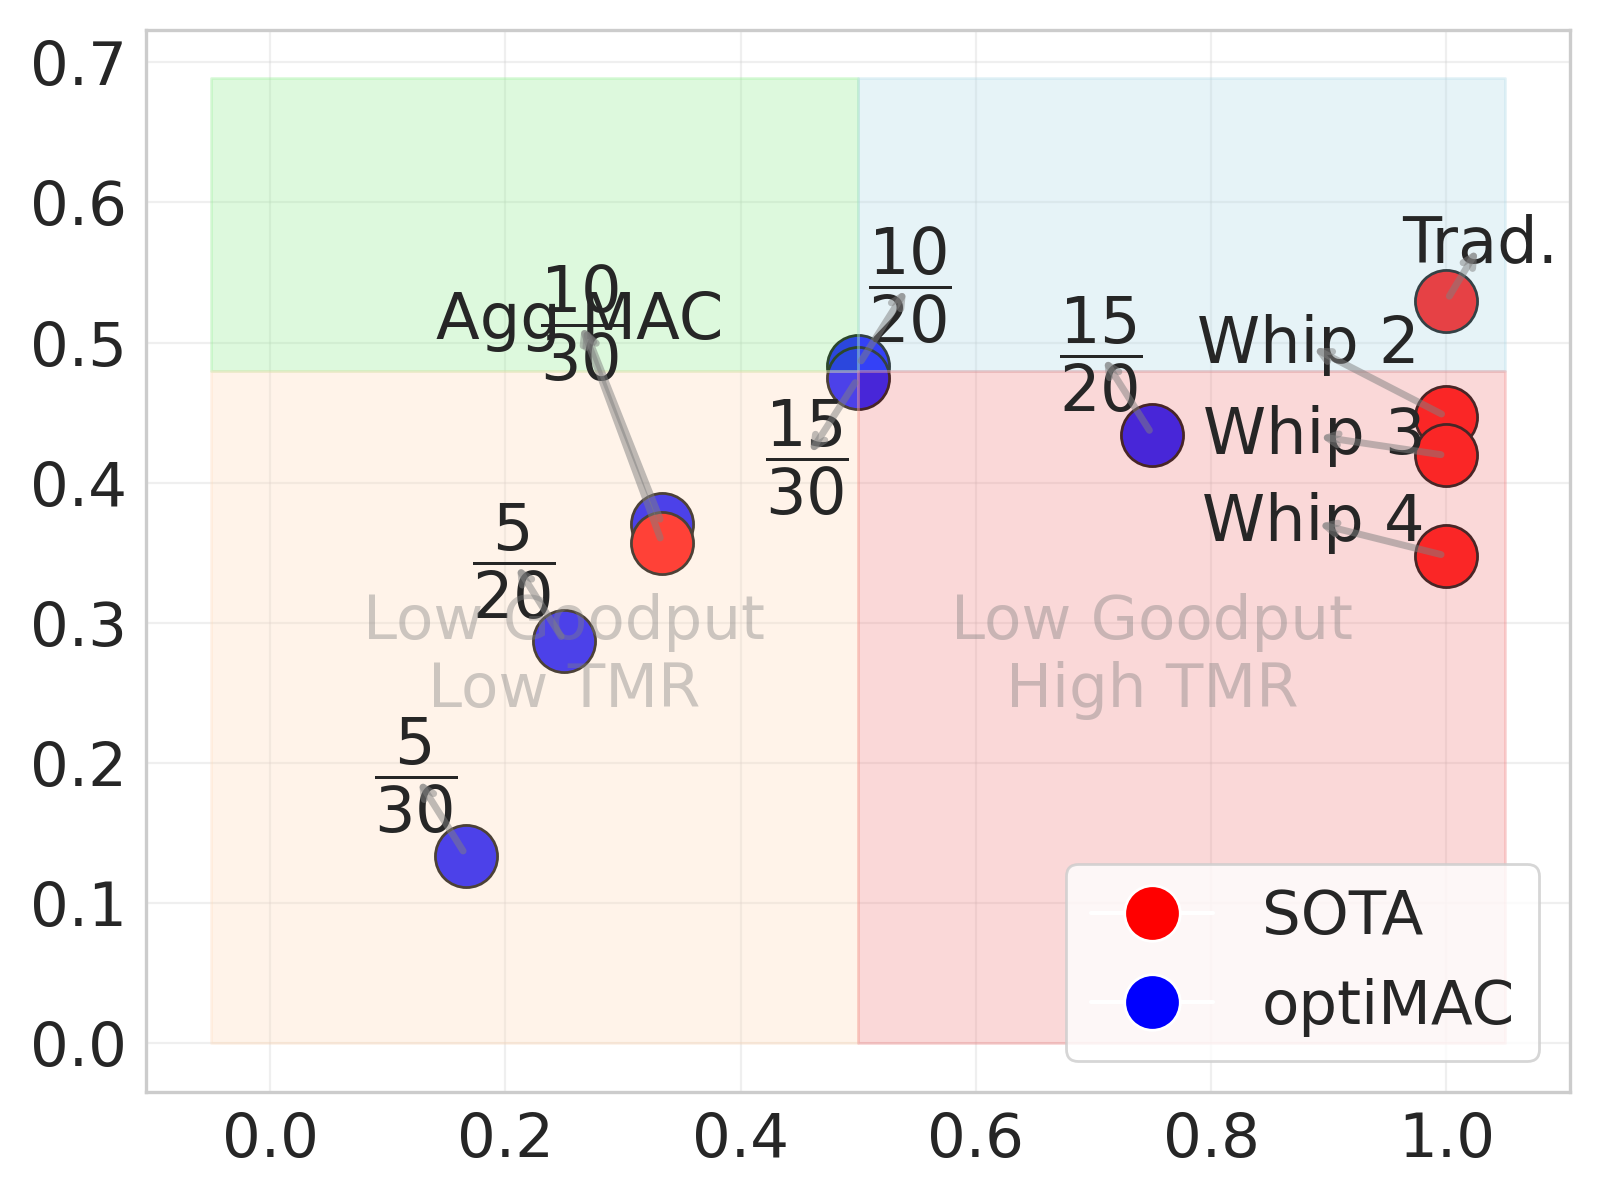
\includegraphics[width=\linewidth]{img/results/5G/0.3G'.png}
         \caption{Attack rate 0.3}
         \label{fig:0.3G 5G}
     \end{subfigure}

     \caption{Goodput (y-axis) vs. TMR (x-axis) of 5G experiments where more than 80\% of Traditional MAC's Goodput is considered high. State-of-the-art (SOTA) includes traditional, progressive, and aggregate MAC vs. the optiMAC.}
     \label{fig:goodput5G}
\end{figure*}
\subsection{Theoretical Goodput (G)}
As similarly defined in~\cite{when_And_How_Aggregate_In_Lossy_Channel}, we define goodput as the ratio of average successfully authenticated bits of messages over the total number of bits transmitted. For a scheme with $m$ messages and $n$ tags, where $|m_i|$ indicated the number of bits of message $i$ and $|t_j|$ indicates the number of bits of tag $j$, the goodput can be defined as follows:
\begin{equation}\label{goodput}
    G = \frac{\sum_{i  = 1}^m Pr(m_i \text{ is verified})|m_i|}{\sum_{i  = 1}^m|m_i| + \sum_{j = 1}^n|t_j|}
\end{equation}
% Moreover we can analyze the Total Tag Length to determine the energy and bandwidth efficiency. the Total Tag Length is defined as follows:
% \begin{equation}
%     \text{Total Tag Length} = \sum_{j=1}^n|t_j|
% \end{equation}
The second term in the denominator represents the total tag length. Both the aggregate MAC and compound MAC schemes reduce the number of tags to improve the goodput. Conversely, it is possible to shorten the tag length without compromising security when multiple tags verify a message (\(A_i > 1\)). Based on the progressive MAC framework, the tag length can be reduced to enhance goodput. 

Moreover, equation~\eqref{goodput} is the expected goodput for statistical analysis; however, for deterministic analysis, the $Pr(m_i \text{ is verified})$ must be replaced by 1 if $m_i$ is verified and 0 otherwise.


\subsection{Strength Number (SN)}
The Strength number SN represents the smallest ratio of messages or tags that, if lost, would prevent the verification of all messages. An upper bound for the strength number is the total number of tags divided by the number of messages, as destroying all tags would result in no verifiable message. If the set consists only of tags, it must include all tags to ensure no message can be verified. However, any tag within this set can be replaced by a message it verifies. If tag-to-message substitutions are selected strategically in a way that for at least two tags, a common message is replaced, the resulting set can potentially have a cardinality less than the number of tags.

Thus, the strength number can be formulated as the minimum number of messages that will make all the tags unusable divided by the number of messages. As a result, let \( \textbf{S} \subseteq \{m_1, m_2, \ldots, m_m\} \) and for any tag, there exists a message in SN that is verified by that tag. 
\begin{equation}
  \textbf{S} = \left\{m_i \mid \quad \forall j, \exists i \quad \text{such that} \quad X_{ij}=1 \right\} 
\end{equation}
The $|\textbf{S}|$ must be minimized to find the strength number. 
% This can be achieved by finding the minimum set of rows in the \( X \) matrix that, when summed, produces a row with all elements greater than or equal to one. To compare different schemes, \( |\textbf{S}| \) can be divided by the total number of messages \( |M| \) to be normalized.
For a given matrix $X$, finding the strength number is similar to the classical set covering the problem with the following formulation. We define a binary variable \( s_i \) for each message.
\begin{equation}
s_i =
\begin{cases} 
1 & \text{if message $i$ is selected} , \\
0 & \text{otherwise}.
\end{cases}
\end{equation}
The mathematical formulation of this set covering problem will be as follows:
\begin{align}
& \text{min} \sum_{i=1}^{m} s_i  &&  \\
& \text{subject to}&& \nonumber\\
& && \sum_{i \in \{i| X_{ij}=1\}} s_i \geq 1, \quad \forall j \in \{1, 2, \ldots, n\} \label{setCoveringConstraint} \\
& && s_i \in \{0, 1\}, \quad \forall i \in \{1, 2, \ldots, m\}
\end{align}
In this formulation, the constraint~\eqref{setCoveringConstraint} guarantees no message will be verified. The objective function is of type cardinality, effectively counting the minimum possible number of messages that guarantee the total failure of the system. Note that the constraint~\eqref{setCoveringConstraint} should only be used for the active tags in $X$. 

Further, $|S|$ must be normalized by the number of messages. Therefore $SN$ is given by:
\begin{equation}
    SN = \dfrac{\text{min}(|S|)}{m},
\end{equation}
where $m$ is the number of messages. The strength number effectively measures the security in terms of availability, representing the percentage of packet loss that results in system failure.

\subsection{Authentication Latency (L)}
Packet latency is when a packet is sent and when the integrity check scheme verifies it. Multiple factors influence it, including implementation details, data rates, and computational power. Additionally, the latency can vary depending on the network layer where the integrity check is deployed. Our objective is to specifically assess the impact of the integrity check scheme on latency compared to traditional MACs under both ideal and attack scenarios. It's important to note that underlying layers—such as the physical, data link, and transport layers—can also contribute to latency, especially when the system is under attack.

To facilitate a relative comparison with traditional MACs, we assume that all tags and messages are correctly received. Under this assumption, authentication latency is the number of additional messages that must be received before a specific message can be authenticated, assuming messages are transmitted sequentially. For instance, if tag $t_j$ verifies messages \( m_{i+1}, m_{i+3}, m_{i+7} \) then \( m_{i+1}\) can be verified only after \( m_{i+\{2,\cdots,7\}} \) are received, which by our definition, the latency is six.

Let's assume that all the messages are sent in order based on their index. For example, \( m_1 \) is sent first and \( m_2 \) is sent afterward. We define the Tag Maximum Index (\textbf{TMI}) vector, where the \( j \)-th entry is the maximum index of the message that the tag \( t_j \) is verifying.
\begin{equation}
TMI_j= \max_{i \in \{i \mid X_{ij} = 1\}} i 
\end{equation}

For example, in the compound MAC shown in Fig.~\ref{fig:compoundMAC}, \( TMI_{j+2} \) corresponding to tag \( t_{j+2} \) equals \( i+6 \), since the the messages that are verified by tag \( t_{j+2} \) are \( m_{i+4}, m_{i+5}, \text{ and } m_{i+6}\).
The authentication latency vector \( \textbf{L} \) is defined as follows:
\begin{equation}
L_i = 
\begin{cases} 
\left(\min_{j \in \{j \mid X_{ij}=1 \}} TMI_j \right)-i & \text{if } A_i > 0 \\
\text{penalty} & \text{otherwise}
\end{cases}
\end{equation}
The penalty is the value assigned if message \( m_i \) is not verified by any tag. For example, the latency vector for the Progressive MAC is all zeros. However, the latency vector for the Compound MAC will be as follows:
$$L = [2, 1, 0, 2, 1, 0, \cdots]$$

\subsection{Latency and Strength Number}
Figure~\ref{fig:otehrMetrics} provides a comparative analysis of the effects of the optimization model on Strength Number (SN) and Latency (L) across different configurations optimized for three distinct attack rates: 0.1, 0.2, and 0.3. Each section corresponds to a specific attack rate and displays bars representing the values of SN (in blue) and L (in red) for various schemes, where each scheme is characterized by a different TMR \( n/m \).
\begin{figure}[h]
    \centering
    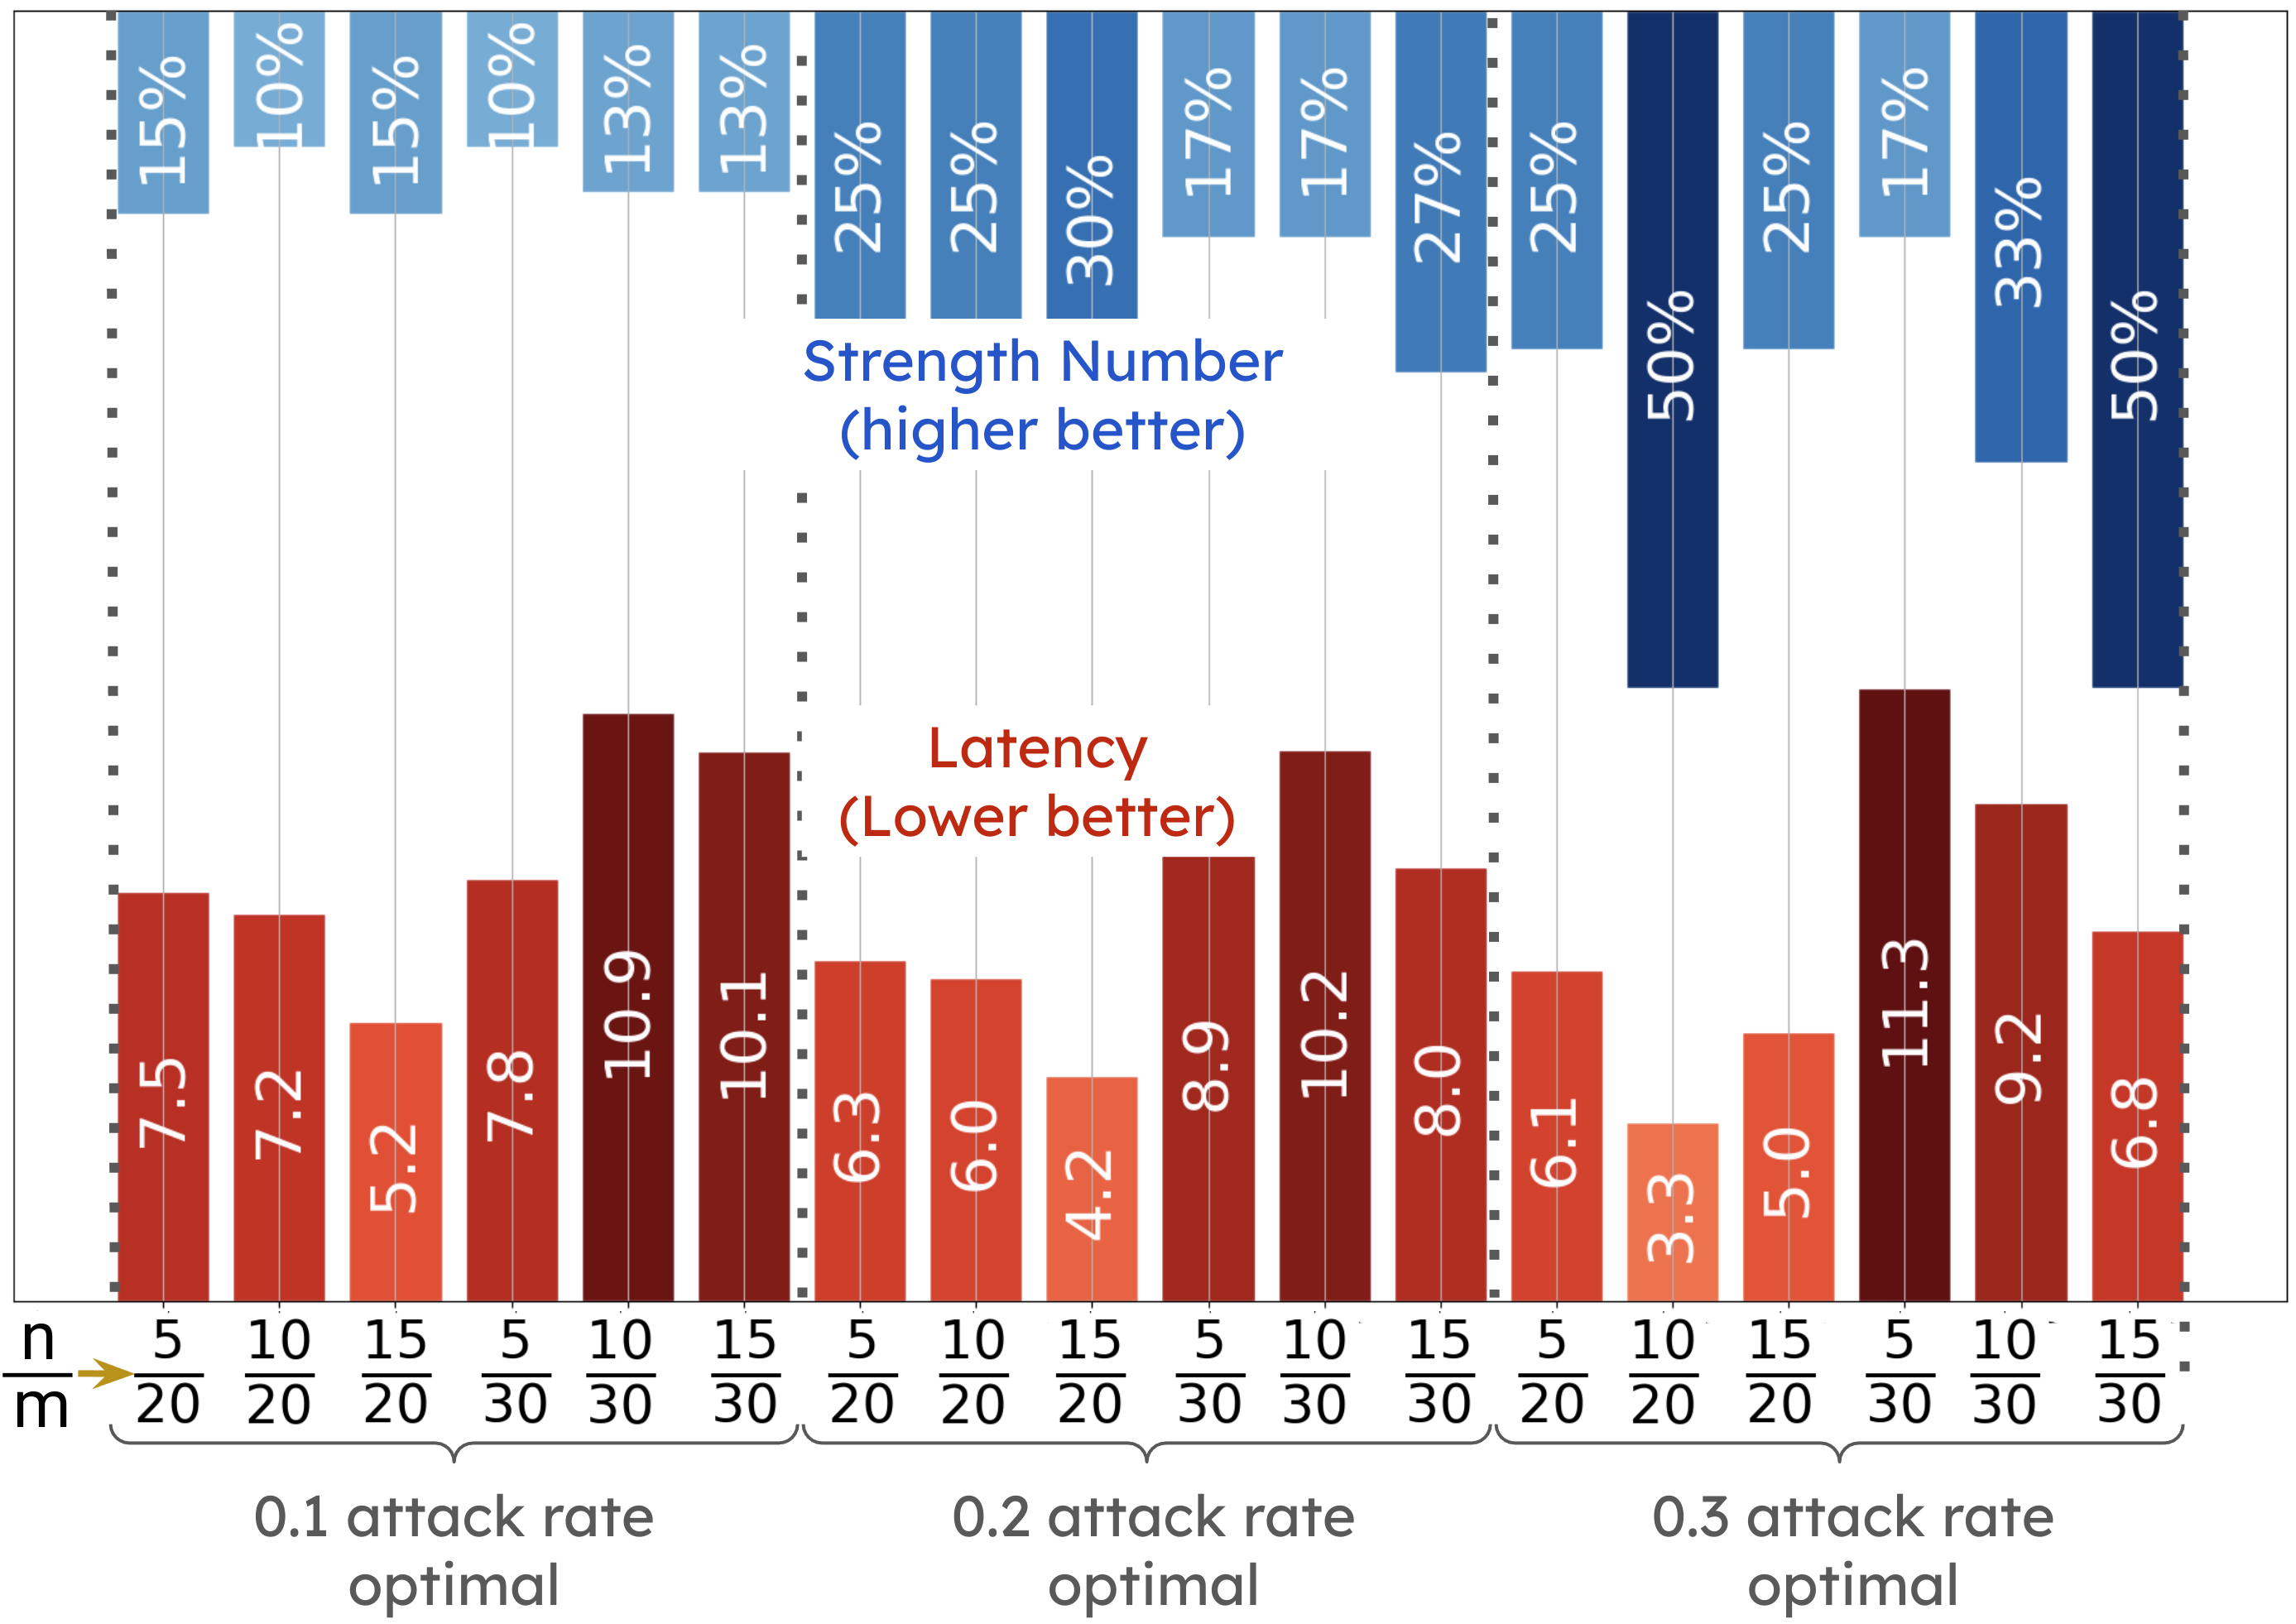
\includegraphics[width=\columnwidth]{img/results/SN vs Latency.png}
    \caption{Strength Number and Latency for the optimal solution by attack rates and Tag-to-Message Ratio ($\frac{n}{m}$).}
    \label{fig:otehrMetrics}
\end{figure}
The Strength Number (SN), represented in shades of blue, measures the percentage of messages that, if lost, will compromise the system's availability, with higher values indicating greater security. As the attack rate increases, the SN generally rises, demonstrating the optimization model's ability to reinforce message-to-tag assignments under more adversarial conditions. For instance, at an attack rate of 0.3, some configurations achieve SN values as high as 33\% and 50\%, reflecting high resilience in challenging environments.

Latency (L), shown in shades of red, represents the delay introduced by the scheme, with lower values indicating better performance. While the optimization model successfully enhances SN, the performance of optimal results in terms of latency and strength is not directly comparable with related works. This limitation is because these additional metrics (latency and SN) were not explicitly represented in the objective function for optimization. Consequently, due to the underlying trade-offs, increased security results in increased latency, as goodput is prioritized.

The optimization model also demonstrates adaptability by reducing dependencies between tags and messages, particularly at higher attack rates, which results in an improved SN even though this metric was not directly optimized. As depicted in Figure~\ref{fig:otehrMetrics}, SN increases with higher attack rates, illustrating the model's capacity to enhance security in response to intensified threats. This visualization effectively highlights the optimization model's impact, showing that it selects configurations with higher SN to maintain security when attack rates rise.


% \section{More Experimental Results}









